\documentclass[12pt]{article}
\usepackage[slovene]{babel}
\usepackage[utf8]{inputenc}
\usepackage[T2A]{fontenc}
\usepackage{amsmath}
\usepackage{amsfonts}
\usepackage{amssymb}
\usepackage[version=4]{mhchem}
\usepackage{stmaryrd}
\usepackage{graphicx}
\usepackage[export]{adjustbox}
\graphicspath{ {./images/} }
\usepackage{physics}
\usepackage{geometry}
\geometry{left=2cm,right=2cm,top=2cm,bottom=2cm}
\usepackage{tikz}
\usetikzlibrary{patterns}

\title{\textbf{Toplotna prevodnost šahovnice iz anizotropnega materiala narezanega pod dvema različnima kotoma}}
\author{Samo Krejan}
\date{september 2025}

\begin{document}
\maketitle

\section{Uvod}

Človeštvo igra šah že vsaj šeststo let, šahovnice pa so v zgodovini uporabljali že za drugačne igre še devetsto let pred tem. Šahovnica ima 64 kvadratih polj razvrščenih v 8 stolpcev in 8 vrstic pobarvane pa so alternirujoče črno in belo (oziroma kakšnih drugih kontrastnih barv). V širšem smislu ima lahko tudi drugačno število polj; 8x8 šahovnici bomo naprej govorili \textit{klasična šahovnica}.


\begin{figure}[htbp]
  \centering

  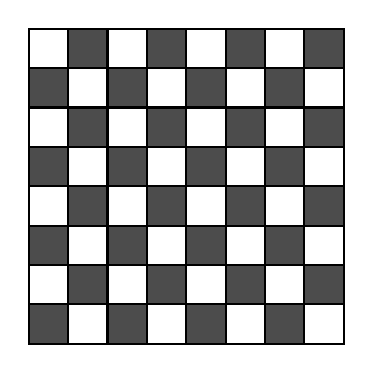
\begin{tikzpicture}[
      square/.style={minimum size=0.5cm, draw=black, thick},
      blacksquare/.style={square, fill=black!70},
      whitesquare/.style={square, fill=white},
      scale=1
    ]
    
    % Draw the 8x8 chessboard
    \foreach \x in {0,...,7} {
      \foreach \y in {0,...,7} {
        % Determine if square should be black or white
        \pgfmathparse{mod(\x + \y, 2) ? "whitesquare" : "blacksquare"}
        \node[\pgfmathresult] at (\x*0.5, \y*0.5) {};
      }
    }
    
    % % Define letters for coordinates
    % \def\letters{{"a","b","c","d","e","f","g","h"}}
    
    % % Add coordinates (letters)
    % \foreach \x in {0,...,7} {
    %   \node at (\x*0.5 + 0.4, -0.4) {\letters[\x]};
    % }
    
    % % Add coordinates (numbers)
    % \foreach \y in {0,...,7} {
    %   \pgfmathsetmacro{\number}{8-\y} % Count down from 8 to 1
    %   \node at (-0.4, \y*0.5 + 0.4) {\number};
    % }
  \end{tikzpicture}
  \caption{klasična šahovnica}
  \label{fig:classical_chessboard}
\end{figure}

Tradicionalno so ljudje izdelovali šahovnice večinoma iz lesa in se izognili potrebi po barvanju, tako da so šahovnico izdelali iz dveh različnih vrst lesa z različnima barvama. Čisto zares pa bi se lahko izdelovalec šahovnic odločil, da bo razlikoval med polji tako, da bo lesne letnice 'črnih' polj postavil pod nek kot glede na stranico, letnice 'belih' pa pod drugačen kot. Taka šahovnica je zelo zanimiva za fizike, saj ima namreč les mnogo lastnosti (med njimi tudi toplotno prevodnost) ki je drugačna če jo opazujemo vzdolž letnic in prečno na letnice. Tako je efektivna toplotna prevodnost celotne šahovnice precej težavna za določit, a ravno to bomo želeli doseči mi.
\newpage
\section{Teoretični uvod}

\newpage
\begin{figure}[h]
  \centering
  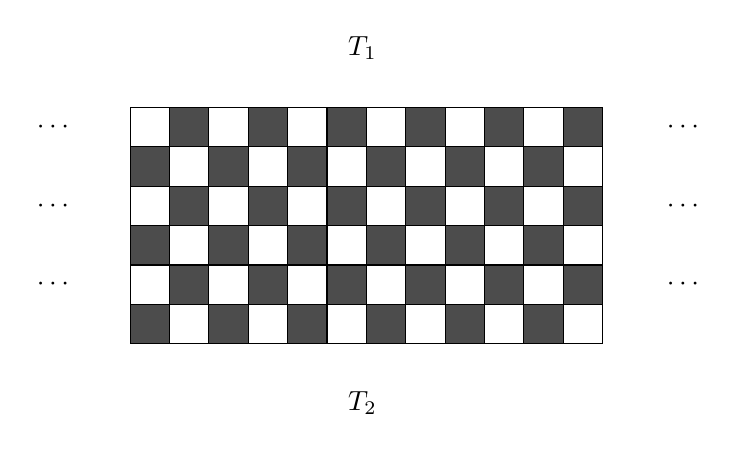
\begin{tikzpicture}[
      square/.style={minimum size=0.5cm, draw=black},
      blacksquare/.style={square, fill=black!70},
      whitesquare/.style={square, fill=white},
      scale=1
    ]
    
    % Draw the 12x6 chessboard
    \foreach \x in {0,...,11} {
      \foreach \y in {0,...,5} {
        % Determine if square should be black or white
        \pgfmathparse{mod(\x + \y, 2) ? "whitesquare" : "blacksquare"}
        \node[\pgfmathresult] at (\x*0.5, \y*0.5) {};
      }
    }
    
    % Add continuation dots on the left
    \foreach \y in {1,3,5} {
      \node at (-1.2, \y*0.5) {$\cdots$};
    }
    
    % Add continuation dots on the right
    \foreach \y in {1,3,5} {
      \node at (12*0.5+0.8, \y*0.5) {$\cdots$};
    }
    
    % Add labels to indicate the pattern continues
    \node[rotate=0] at (2.7, 3.5) {$T_1$};
    \node[rotate=0] at (2.7, -1) {$T_2$};
  \end{tikzpicture}
  \caption{Skica problema (šahovnica se nadaljuje neskončno v levo in desno)}
  \label{fig:wide_chessboard}
\end{figure}





\end{document}